% Drawing 69/06-13 -- folder 69, batch 06, archive page 119 (PDF page 120).
% Transcription: en bas, plusieurs courbes fermées : un disque partagé en trois régions numérotées 1, 2, 3 ; deux ovales emboîtés, parcourus de flèches ; un petit cercle avec son centre, relié par un segment à un point $a$
% Kind: closed curves: disk in three regions, nested ovals with arrows, small circle joined to a. Method 2 (schematic redraw from the facsimile). Status: partial.
% Notes: Upside-down page (rotated). Bottom: a disk cut into three regions 1, 2, 3; two nested ovals traversed by arrows; a small circle with its centre, joined by a segment to a point a; other closed curves (left) drawn roughly. Approximate.
% Coordinates: 1 unit = 1 mm = 1/100 of the crop width (bbox in page fractions: [0.08, 0.15, 0.95, 0.86]).
% Redrawn by Claude (claude-opus-5-5), issue #73, 2026-11-07; not checked by a human; not compiled (no TeX in the session).
% Rights: reproduces part of the work -- behind RENDER_TRANSCRIPTS, never published by itself.
\documentclass[tikz,border=3pt]{standalone}
\usepackage{amsmath,amssymb}
\usetikzlibrary{patterns,arrows.meta}
\tikzset{pencil/.style={black!45}, struck/.style={black!35}, mark/.style={circle,draw,inner sep=1.3pt}, pt/.style={circle,fill,inner sep=0.9pt}, opt/.style={circle,draw,fill=white,inner sep=1.1pt}}
\begin{document}
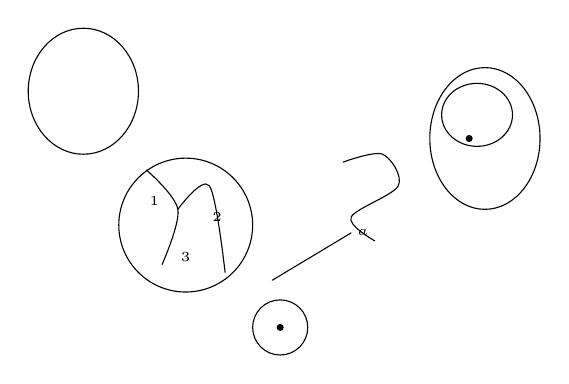
\begin{tikzpicture}[x=1mm,y=1mm,line cap=round,line join=round,font=\scriptsize]
\draw (41,-93) circle[radius=8.5];
\draw plot[smooth, tension=0.55] coordinates {(36,-86) (40,-91) (38,-98)};
\draw plot[smooth, tension=0.55] coordinates {(40,-91) (44,-88) (46,-99)};
\node[inner sep=1pt] at (37,-90) {\tiny $1$};
\node[inner sep=1pt] at (45,-92) {\tiny $2$};
\node[inner sep=1pt] at (41,-97) {\tiny $3$};
\draw (79,-82) ellipse[x radius=7, y radius=9];
\draw[-{Stealth[length=2mm]}] (78,-79) ellipse[x radius=4.5, y radius=4];
\node[pt] at (77,-82) {};
\draw (53,-106) circle[radius=3.5];
\node[pt] at (53,-106) {};
\draw (52,-100) -- (62,-94);
\node[inner sep=1pt] at (63.5,-94) {\tiny $a$};
\draw (28,-76) ellipse[x radius=7, y radius=8];
\draw plot[smooth, tension=0.55] coordinates {(61,-85) (66,-84) (68,-88) (62,-92) (65,-95)};
\end{tikzpicture}
\end{document}
